
\chapter[Barycentric coordinates computation]{Barycentric coordinates \\computation}
\label{app:barycentric_}

Let $\mathit{t} = \mathbf{A}\mathbf{B}\mathbf{C}$ be a triangle (see Figure \ref{fig:bar}(a)). 
The barycenter $\mathbf{P}$ of $t$ is the intersection of the three medians, meaning that if we put three equal masses $w$ at the vertices of the triangle, and the triangle is parallel to the ground, $P$ is the center of gravity, where the forces are in equilibrium.

Whether we move the point $P$ inside the triangle, we need to put three different weights $w_1$, $w_2$ and $w_3$ at the three in order to keep the equilibrium (see Figure \ref{fig:bar}(b)). 
These three weights are named \emph{barycentric coordinates}.
With the barycentric coordinates we can express the point $P$ as:
\begin{equation}
\label{eq:bar_mass}
 \mathbf{P} = \frac{1}{\sum_i w_i}  w_1 \mathbf{A} + w_2 \mathbf{B} + w_3 \mathbf{C}.
\end{equation}

\begin{figure}[bt]
 \begin{tabular}{cc}
  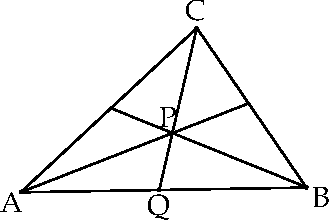
\includegraphics[width=0.45\textwidth]{./img/ch-appendix/barycentric01}&
  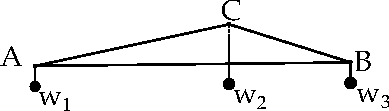
\includegraphics[width=0.45\textwidth]{./img/ch-appendix/barycentric02}\\
  (a)&(b)
 \end{tabular}
 \caption{Triangle and barycentric coordinates: 
 (a) the point $\mathbf{P}$ is the barycenter of the triangle 
 $\mathbf{ABC}$ result of the intersection of the medians; 
 (b) the barycentric coordinates can be visualized as masses applied to the vertices $\mathbf{A}$, $\mathbf{B}$ and $\mathbf{C}$.
 }
 \label{fig:bar}
\end{figure}

To simplify this expression, barycentric coordinates are usually normalized such that:
\begin{equation}
  w_1 + w_2 + w_3 = 1.
\end{equation}

\section{Areal coordinates}
We can rewrite Equation \eqref{eq:bar_mass} as:
\begin{equation}
\label{eq:bar_mass2}
 (w_1 + w_2 + w_3) \mathbf{P} =  w_1 \mathbf{A} + w_2 \mathbf{B} + w_3 \mathbf{C}.
\end{equation}
\begin{equation}
\label{eq:bar_mass2}
 (w_1 + w_2 + w_3) \mathbf{P} =  (w_1  + w_2) \mathbf{Q} + w_3 \mathbf{C},
\end{equation}
with $\mathbf{Q}$ defined as the center of mass of $A$ and $B$,
\begin{equation}
 \mathbf{Q} = \frac{w_1 \mathbf{A} + w_2 \mathbf{B}}{w_1 + w_2},
\end{equation}

Since the  distances from the endpoint to the center of mass are inversely proportional to the masses:
\begin{equation}
 \frac{w_1}{w_2} = \frac{\mathbf{BQ}}{\mathbf{AQ}}.
\end{equation}
The triangles $\mathbf{QBC}$ and $\mathbf{QAC}$ shares the same height and the bases are respectively $\mathbf{BQ}$ and $\mathbf{AQ}$ so:
\begin{equation}
 \frac{\mathbf{BQ}}{\mathbf{AQ}}  = \frac{\mathbf{QBC}}{\mathbf{QAC}}.
\end{equation}
Analogously, $\mathbf{QBP}$ and $\mathbf{QAP}$ shares the same base, while the heights are $\mathbf{BQ}$ and $\mathbf{AQ}$:
\begin{equation}
  \frac{\mathbf{QBC}}{\mathbf{QAC}} =  \frac{\mathbf{QBP}}{\mathbf{QAP}} = 
  \frac{\mathbf{QBC-QBP}}{\mathbf{QAC-QAP}} = \frac{\mathbf{CBP}}{\mathbf{CAP}}.
\end{equation}
Therefore this equation holds:
\begin{equation}
  \frac{w_1}{w_2} =  \frac{\mathbf{CBP}}{\mathbf{CAP}}.
\end{equation}
Let remember that barycenter coordinates are normalized, since only the ratio are well defined; for the same reason we can derive that the barycentric coordinate associated to a vertex is proportional to the area of the respective opposite triangle.
In particular, to obtain the normalized coordinate $w_1$, $w_2$ and $w_3$ we have:
\begin{align}
\label{eqn:eqlabel}
\begin{split}
 w_1 =  \frac{\mathbf{CBP}}{\mathbf{ABC}} \\
 w_2 =  \frac{\mathbf{CAP}}{\mathbf{ABC}} \\
 w_3 =  \frac{\mathbf{ABP}}{\mathbf{ABC}} 
\end{split}.
\end{align}


For this reason the barycentric coordinates are also referred to as \emph{areal coordinates}, and their computation from Cartesian coordinates exploits this property and the relation $A_{V_1V_2V_3} = \frac{\| \overrightarrow{V_1V_2} \times \overrightarrow{V_1V_3}  \|}{2}$.










% 
% float orientPoint(vec2 v0, vec2 v1, vec2 p){
%   mat2 m;
%   m[0][0] = (v1.x - v0.x);  m[0][1] = ( p.x - v0.x);
%   m[1][0] = (v1.y - v0.y);  m[1][1] = ( p.y - v0.y);
% 
%   return m[0][0] * m[1][1] - m[0][1] * m[1][0];
% }
% 
% vec3 barycentricCoordMine(vec2 p, vec2 p0, vec2 p1, vec2 p2){
%   vec2 v0, v1, v2;
%   //First Check if triangle is counter-clockwise
%   if(orientPoint(p0, p1, p2) > 0){
%     v0 = p0;
%     v1 = p1;
%     v2 = p2;
%   }else{
%     v0 = p0;
%     v1 = p2;
%     v2 = p1;
%   }
%   // Compute barycentric coordinates w.r.t pt1
%   vec3 barycentricCoordinates;
% 
%   float areaTrtwice = orientPoint(v0, v1, v2);
% 
%   if(areaTrtwice!=0){
%     barycentricCoordinates.x = orientPoint(v0, v1, p)/areaTrtwice;
%     barycentricCoordinates.y = orientPoint(v1, v2, p)/areaTrtwice;
%     barycentricCoordinates.z = orientPoint(v2, v0, p)/areaTrtwice;
%   }else {
%    return vec3(-1.0);
%   }